\documentclass[tikz, border=5mm]{standalone}

\usetikzlibrary{arrows.meta,decorations.markings,fit,calc, positioning}

\definecolor{componentColor}{RGB}{210,210,210}
\definecolor{systemColor}{RGB}{230,230,230}

\tikzset{component/.append style={fill=componentColor, align=center, draw, minimum width=2cm, minimum height=1.5cm, rounded corners=.3cm}}
\tikzset{system/.style={component, fill=systemColor, rounded corners=0cm}}

\tikzstyle{arrow} = [-{Latex[scale=3.0]}]
\tikzset{arrowLabel/.append style={minimum height=.25cm, draw=none}}
\begin{document}

	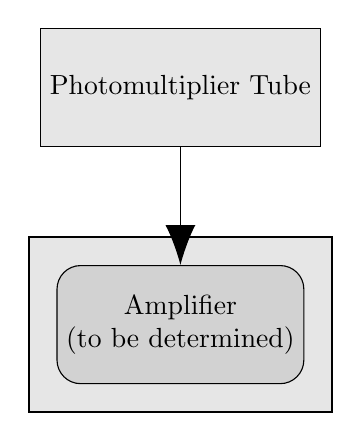
\begin{tikzpicture}[node distance=1.5cm and 3cm]
	% Nodes
	\pgfdeclarelayer{background}
	\pgfsetlayers{background,main}
	
        \node (photomultiplier) [system] {Photomultiplier Tube};	
		
        \node (amplifier) [component, below=of photomultiplier] {Amplifier\\ (to be determined)};	

		\begin{pgfonlayer}{background}
		\node[system, draw, thick, inner xsep=1em, inner ysep=1em, fit= (amplifier)] {};
		\end{pgfonlayer}
	    

		% Connectors
		\begin{scope}[->]
		
		\draw [arrow] (photomultiplier) --(amplifier);



	\end{scope}

\end{tikzpicture}
\end{document}